%%% Ne pas modifier jusqu'à la ligne 25
\documentclass[a4paper,12pt]{book}
\usepackage[utf8]{inputenc}
\usepackage[french]{babel}
%%\usepackage{CJK}
\usepackage{yhmath}
\usepackage[left=2cm,right=2cm,top=3cm,bottom=2cm, headheight=1.5cm,headsep=1.5cm]{geometry}
%%\usepackage{CJKutf8}
\usepackage{amsfonts}
\usepackage{amsmath,amsfonts,amssymb,dsfont}
\usepackage{graphicx}
\usepackage{enumitem}		%\enumerate-resume
\usepackage[colorlinks=true,unicode={true},hyperindex=false, linkcolor=blue, urlcolor=blue]{hyperref}
\newcommand{\myref}[1]{\ref{#1} page \pageref{#1}}

\addto\captionsfrench{\def\tablename{Tableau}}  %légendes des tableaux
\renewcommand\thesection{\Roman{section}~-~} 
\renewcommand\thesubsection{\Roman{section}.\Alph{subsection}~-~} 
\renewcommand\thesubsubsection{\Roman{section}.\Alph{subsection}.\arabic{subsubsection}~-~} 

\newcommand{\conclusion}[1]{\newline \centerline{\fbox{#1}}}

\setcounter{secnumdepth}{3}
\parindent=0pt

\usepackage{fancyhdr}
\pagestyle{fancy}

\lhead{SJTU-ParisTech} 
%%%%%%%%%%%%%%%%%%%%%%%%%%%%%%%%%%
\chead{TR4}
\rhead{Daniel 518261910024}

\begin{document}
\renewcommand{\labelitemi}{$\blacktriangleright$}
\renewcommand{\labelitemii}{$\bullet$}


\section{la différence de marche}
\begin{figure}[h]
    \begin{center}
    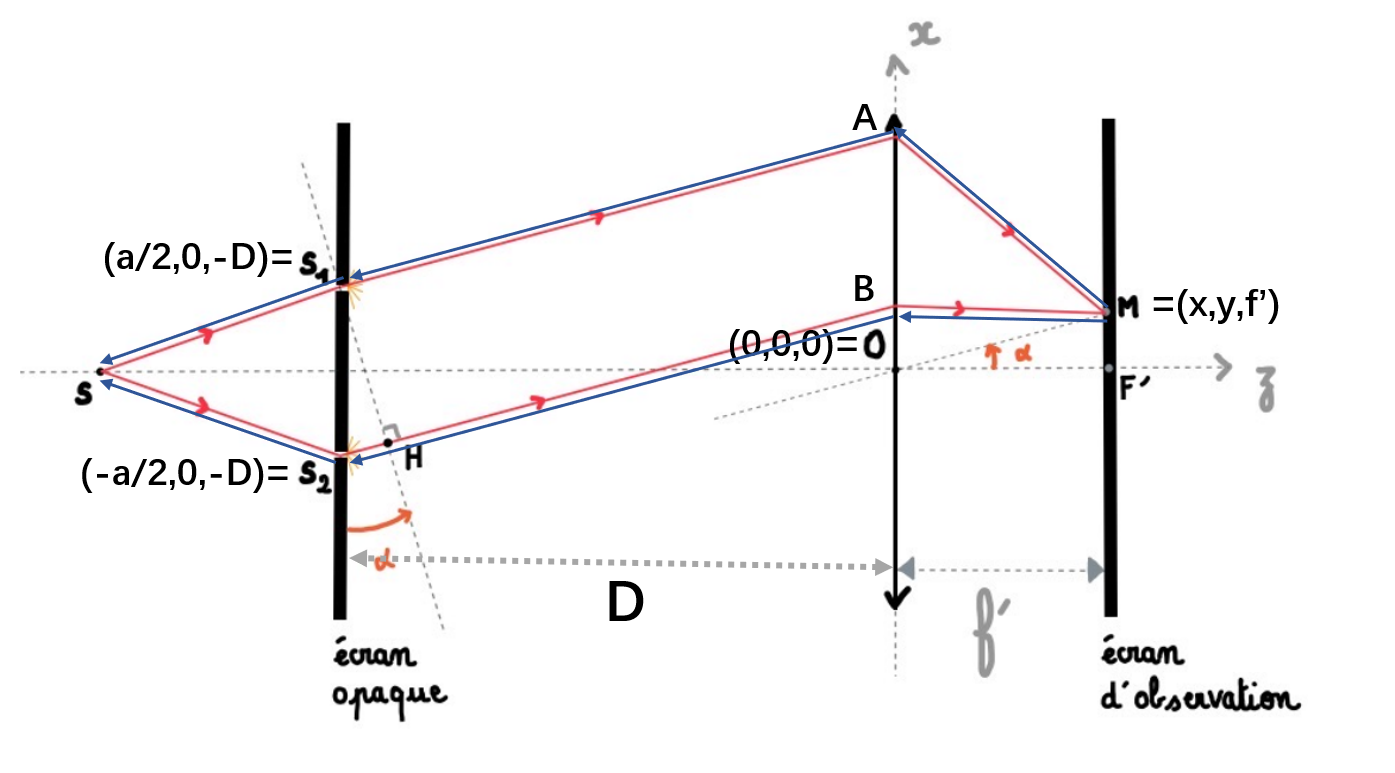
\includegraphics[scale=0.7]{tr4.png}
    \end{center}
    \caption{Expérience des trous de Young}
\end{figure}
On commence par $$\delta_{2/1}(M)=(SM)_2-(SM)_1$$
Supposons que l'expérience est fait dans un milieu homogène d'indice de fraction $n$: 
$(SM)_1=n*SM=n*S_1M+n*SS_1=(S_1M)+(SS_1)$, de même, $(SM)_2=(S_2M)+(SS_2)$, on arrive à 
$$\delta_{2/1}(M)=(SS_2)-(SS_1) + (S_2M)-(S_1M) $$
Car $S_1$ et $S_2$ sont symmétrique par rapport à l'axe $O_z$ sur lequelle $S$ se trouve, 
on a $SS_1=SS_2$, donc $(SS_1)=(SS_2)$, d'où
$$\delta_{2/1}(M)=(S_2M) - (S_1M)=(S_2H)+(HM)-(S_1M)$$
Par principe du retour inverse de la lumière, on peut considerer les deux rayons en bleu, 
qui sont issus de M et qui suivent le même direction que les rayons en rouge, mais de sens opposites. 
On a donc 
$$
\phi(S_1)=\phi(M)+(MS_1)
$$
$$
\phi(H)=\phi(M)+(MH)
$$
Et selon théorème de Malus, puisque $S_1H$ est perpendiculaire aux deux rayons parallèles entre eux, 
$S_1$ et $H$ sont sur la même surface d'onde, c'est à dire: $\phi(S_1)=\phi(H)$. 
On a donc $\phi(M)+(MS_1)=\phi(M)+(MH)$, d'où $(MS_1)=(MH)$, donc 
$$
\delta_{2/1}(M)=(S_2H)=\overline{S_2H}
$$
lorsque on fait l’expérience dans le vide($n=1$). On utilise la mesure algébrique ici pour faire des calculs suivants car 
$\overline{S_2H}$ est $\delta_{2/1}(M)$ sont de même signe (Si $M$ est au-dessus de $Oz$, ils sont tous positifs, 
et si $M$ est au-dessous, ils sont tous negatifs).

Puisque $\stackrel{\longrightarrow}{S_2H}$ est le projection de $\stackrel{\longrightarrow}{S_2S_1}$ sur $\stackrel{\longrightarrow}{S_2B}$, qui est forcément parallèle à $\stackrel{\longrightarrow}{OM}$, on a donc 
\begin{align*}
    \overline{S_2H}&=\frac{\stackrel{\longrightarrow}{S_2S_1}\cdot\stackrel{\longrightarrow}{S_2B}}{||\stackrel{\longrightarrow}{S_2B}||}\\
    &=\frac{\stackrel{\longrightarrow}{S_2S_1}\cdot\stackrel{\longrightarrow}{OM}}{||\stackrel{\longrightarrow}{OM}||}\\
    &=\frac{(a,0,0)\cdot (x,y,f')}{||(x,y,f')||}\\
    &=\frac{ax}{\sqrt{x^2+y^2+f^{'2}}}\\
    &=\frac{ax}{f'}\left(1+\left(\frac{x}{f'}\right)^2+\left(\frac{y}{f'}\right)^2\right)^{-\frac{1}{2}}
\end{align*}
Si on fait l'observation proche de l'axe est à une grande distance: 
$|x|\ll f'$ et $|y| \ll f'$, donc $\left(\frac{x}{f'}\right)^2+\left(\frac{y}{f'}\right)^2 \ll 1$. 
Par développement limité à l'ordre $0$, on a 
$\left(1+\left(\frac{x}{f'}\right)^2+\left(\frac{y}{f'}\right)^2\right)^{-\frac{1}{2}}=1$. 
Finalement, la différence de marche est $\boxed{\delta_{2/1}(M)=\overline{S_2H}=\frac{ax}{f'}}$







\end{document}